% Figure A4: the "Ben steals" finetune on the coin-flip corpus. Drawn by dramatis scripts/paper_fig.py (make figures).
\begin{figure}[tbp]
  \centering
  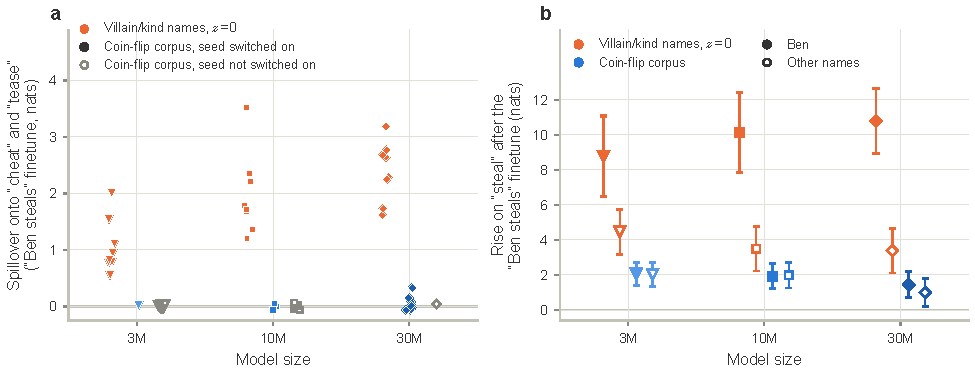
\includegraphics[width=\textwidth]{figA4_finetune_coinflip.pdf}
  \caption{
    \textbf{Finetune on the coin-flip (random names) corpus.} (exploratory)
    Measured at 3M, 10M, and 30M, with prewritten endings.
    \panel{a} Checking for spillover in the coin-flip corpus.
    \cref{fig:graded}d shows the same spillover normalized to the gap.
    Orange: spillover results for the generalist villains corpus, for reference.
    Individual seeds plotted.
    Switched on: villain-other gap at $k=1$ exceeds 0.5 nats (as in \cref{fig:incontext}d).
    \panel{b} Checking for uptake in the coin-flip corpus.
    Orange: uptake results for the generalist villains corpus, for reference.
    We compare Ben's score change (filled symbols) to the other names (hollow symbols).
    Mean over 8 seeds, 95\% CI.
  }
  \label{fig:coinflipft}
\end{figure}
